\section{An extended Model}

After asserting that a deep reinforcement learning agent can navigate the state space easily, we extend the model to address the issues we found in the simple model presented in section \ref{sec:model1}. First we want to address that women should not permanently withdraw from the labour force. Second the log-function used for the sub-utilities caps the utility very hard, which implies that for very small perturbations of $\beta_L$ makes the agent substitute into one of the extremes, working 45 hours exclusively or working 0 hours exclusively. They agent should ideally be more balanced, therefore the functional form of the sub-utilities should have a steeper curvature. Since the other papers have suggested that children do not take a uniform amount of time from mothers leisure over the life cycle, I track the age of the children, such that a functional form of the amount of time used on children can vary by the age of the child:

\begin{equation}
    U_t = \beta_L L_{t}^\zeta + \beta_Y Y_t^{\zeta}
\end{equation}

The fertility process should also be extended. I now assume that each household can have a maximum of four kids. I track whether how many kids the family has, and the associated age. Still in each period the number of children in the household can increment by one.

\begin{equation}
    K_{t+1} = K_t+ \psi_t, \qquad \psi_t \mid Q_t \sim Bernoulli (p_\psi(Q_t))
\end{equation}

However i now let $B^\top$ be a vector of size 4 equal to the maximum number of children. Furthermore i let the vector $C^\top$ denote the individual age of the children also of size 4. This implies the for index $i$ of vector $K$ implies the $i$'th child, index $i$ of vector $C$ implies the same child's corresponding age.

\begin{equation}
    B_t[i]  = \begin{cases}
        1 & \text{if }  i \leq K_t \\
        0 & \text{else}
    \end{cases}
\end{equation}

and the age vector is defined as:

\begin{equation}
    C_{t+1} = C_t + B_{t+1}
\end{equation}

So that the age of the children only increments if and only if the children lives.

Finally the utility part of the model need to be adjusted to take into account the number of hours used pr. child. Let $J$ denote the number of hours used on children. Using the numbers found by \parencite{ekert-jaffe_time_2015} one can say that for children below age 3 takes 10 hours pr week, children in the age 3 up to age 16 takes 3.5 hours pr. week, and children above takes 0 hours of leisure pr. week for women. 

\begin{equation}
    J_t = \sum_{i=1}^4 \begin{cases}
        0.0 & \text{if } B_t[i] = 0 \\
        10.0 & \text{if } B_t[i] = 1 \land C_t[i] < 3 \\
        3.5 & \text{if } B_t[i] = 1 \land 3 \geq C_t[i] < 16 \\
        0 & \text{if } B_t[i] = 1 \land  16 \geq  C_t[i] 
    \end{cases}
\end{equation}

Another thing to address is, that empirically women tend to work less when they are young (in the age of 18 to 30), gradually increasing the number of working hours as shown in figure \ref{fig:dqi_model1_average_path_sim_vs_empirical}. This is probably a consequence of education. Looking to figure \ref{fig:educ_empirical}, it could appear to be a consequence of women doing full time education, not having the time to work (more than a few hours a week) that could explain the result. To address this problem I add to the model an education parameter. In this setup the education does not add to higher salary instead it only goes in the model as additional time spent. Education is assumed to be exogenous, and over the life cycle the women will with some probability be done with education, not to return ever again to the education system. Using \textbf{FOLK1A} from Statistics Denmark i find the total number of women in a given age group. The total number of women for a given age group doing full time education is found in the source \textbf{UDDAKT10} also from Statistics Denmark. I fit this with a linear regression and find a path linearly decreasing the number of women doing full time education This can be seen in Figure \ref{fig:prob_educ_full_time}. I model the education the following way:

\begin{figure}[ht]
\begin{subfigure}{.5\textwidth}
  \centering
  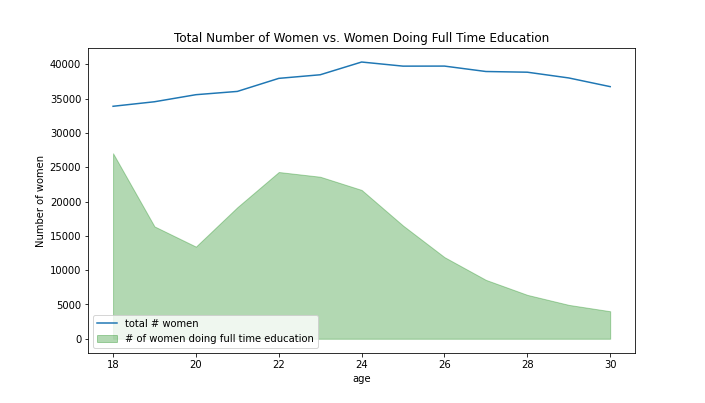
\includegraphics[width=1\linewidth]{figures/total_women_vs_education.png}
  \caption{FTE vs. Total Number of Women}
  \label{fig:educ_empirical}
\end{subfigure}%
\begin{subfigure}{.5\textwidth}
  \centering
  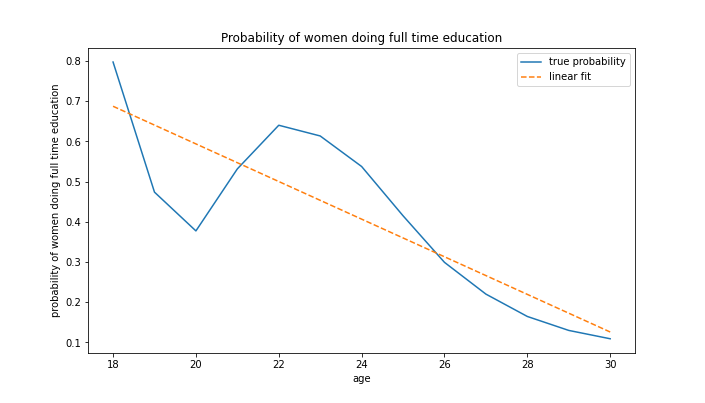
\includegraphics[width=1\linewidth]{figures/prop_women_doing_full_time_education.png}
  \caption{Fraction of Women in FTE vs. Linear Fit}
  \label{fig:prob_educ_full_time}
\end{subfigure}
    \caption{Women and Full Time Education (FTE)}
    \label{fig:educ_women}
\end{figure}

\begin{equation}
    E_{t+1} = E_{t} \cdot \iota_t, \qquad \iota_t \mid Q_t \sim  Binomial(p_{\iota}(Q_t))
\end{equation}

So in each period with some probability $E^{prob}_t \equiv p_{\iota}(Q_T)$ the women will end full time education. Both $E$ and $E^{prob}_t$ is part of the state space. Since women do full time education i let assume that the time used on full time education is 37 hours pr. week.

It is assumed for simplicity that human capital accumulation does not depreciate or accumulate when the agent is under full time education:

\begin{equation}
    G_{t+1} = 
    \begin{cases}
        G_t(1 - \delta) + \frac{H_t}{37}, & \text{if } E_t > 0 \\
        G_t & \text{else}
    \end{cases}
\end{equation}


Finally note that the utility is calculated pr. week basis instead of on an annual basis. This is again done, such that the sub utilities, do not squash the values to hard, as was the case in model 1, making estimating of the model very hard, allowing small perturbations of $\beta_L$ having to much effect. Also compared to the original model $f^M(Q_t)$ now represents the number weekly total income of the husband rather than the annual.

\begin{equation}
    L_t = 24 \cdot 7 - H_t - J_t - E_t \cdot 37
\end{equation}

Since education is coupled with a transfer from the state in the danish context this is added as well, such that the household will a transfer of $tr = \frac{6000 DKK \times 12}{52} \approx 1400 DKK$ each week from the government, while the women is studying. This ratio is approximately doubled if the women gets a child during the education \parencite{noauthor_satser_nodate-1}. The total income of the household is equal to:

\begin{equation}
    Y_t = H_t \cdot W_t + f^M(Q_t) + E_t (tr + \mathbf{1} \{ K_t > 0 \} \cdot tr)  
\end{equation}


Summarizing the model; using a lot of the framework from the simple model a couple of extensions is made. The state space is now of 14 dimensions containing $(Q)$ age, $(G)$ human capital, $(Z)$ idiosyncratic wage path, $(K)$ the number of children in at time $t$ in the household, a vector of size four $(B)$ corresponding to the number of children the household have contain, a vector of size 4 $(C)$ containing the age of the individual children, a dummy $(E)$ that indicates if the women is under education, and lastly $E^{prob}$ a number between 0 and 1 that indicates the probability of staying being enrolled in full time education next period. The action space is slightly tweaked to contain $\{ 0, 15, 25, 37\}$ representing the discreet choices of hours the woman can choose to work. This formulation is closer to that of \textcite{francesconi_joint_2002}, where he only considers the choices \{nonwork, part-time, full-time\}. In the formulation of this extended model, there is distinguished between two types of part time work; 15 and 25 hours a week. The model specification is:

\begin{equation}
    \textbf{State space: }\statespace = \R^2 \times \{0, 1, 2, 3, 4\} \times \{18, 19, \cdots , 60\} \times \{0, 1\}^4 \times \{0, 1, \cdots, 18\}^4 \times \{0,1\} \times [0, 1]
\end{equation}

\begin{equation}
    \textbf{Action space: }\actionspace = \{0, 15, 25, 37\}
\end{equation}

Additionally the model contains the following parameters: $\alpha=, \eta_G = 0.164, \eta_{G^{2}}=0.015, \delta, \sigma_\epsilon = 15.11, \beta_L, \beta_Y = 1, W_{min} = 120, tr = 1600, \zeta=0.5$. Using the values of the Mincer equation from the parameter tuning performed earlier! A recursive formulation of the model is presented below:


IKKE FÆRDIG MED RECURSIVE FORMULERING!

\begin{align}
    U_t(L_t, Y_t) &= \beta_L L_t^{\zeta} + \beta_Y Y_t^{\zeta}\\
    L_t(K_t, H_t, J_t, E_t) &= 24 \cdot 7 - H_t - J_t - E_t \cdot 37\\
    \log \tilde{W}_t (G_t) &= \alpha + \eta_G G_t + \eta_{G^2} G_t^2 \\
    W_t(\tilde{W}_t, Z_t) &= \max(W_{min} , \tilde{W}_t  + Z_t)  \\
    Y_t(Q_t,H_t, W_t, E_t, K_t) &= 46 \cdot H_t \cdot W_t + f^M(Q_t) +  E_t (tr + \mathbf{1} \{ K_t > 0 \} \cdot tr)\\
    J_t (B_t, C_t) &= \sum_{i=1}^4 \begin{cases}
        0.0 & \text{if } B_t[i] = 0 \\
        10.0 & \text{if } B_t[i] = 1 \land C_t[i] < 3 \\
        3.5 & \text{if } B_t[i] = 1 \land 3 \geq C_t[i] < 16 \\
        0.0 & \text{if } B_t[i] = 1 \land  16 \geq  C_t[i] 
    \end{cases} \\
    B_t[i] (K_t) &= \begin{cases}
        1 & \text{if }  i \leq K_t \\
        0 & \text{else}
    \end{cases}
\end{align}

Law of motion:

\begin{align}
    Q_{t+1}(Q_t) &= Q_t \\
    K_{t+1}(K_t, Q_t)  &= K_{t} + \psi_t, \qquad \psi_t \mid Q_t \sim Bernoulli(p_\psi(Q_t))  \\
    Z_{t+1}(Z_t) &= Z_t + \epsilon_t, \qquad \epsilon_t \sim \ndist(0, \sigma_\epsilon)\\
    G_{t+1}(G_t, H_t, E_t) &= 
    \begin{cases}
        G_t(1 - \delta) + \frac{H_t}{37}, & \text{if } E_t > 0 \\
        G_t & \text{else}
    \end{cases} \\
    C_{t+1}(C_t, B_{t+1}) &= C_{t} + B_{t+1} \\
    E_{t+1}(E_t, Q_t) &= E_t \cdot \iota_t, \qquad \iota_t \mid Q_t \sim Binomial(p_\iota(Q_t))
\end{align}


